\chapter{REFERENCIAL TEÓRICO}

\section{Inovação para o desenvolvimento rural}


O empreendedorismo não consiste apenas na criação de empresas. Ser empreendedor vai além de ter seu próprio negócio, e implica em uma visão de mundo diferente, uma mudança de paradigma, de pensamento. Garcia \cite{garcia_formacao_2000} define o empreendedorismo como sendo a habilidade de criar e de construir algo, a partir do nada, sendo o empreendedorismo um ato humano nascido da criatividade. O empreendedor é um constante inovador, sendo aquele que está sempre em busca de soluções, que consegue enxergar nas oportunidades, tendo iniciativa e sendo proativo e visionário. Dessa forma, podendo contribuir para introduzir inovações na empresa na qual trabalha, ajudar a solucionar problemas da sua cidade, entre outras possibilidades que se fazem presentes a partir do momento que um comportamento empreendedor é desenvolvido, \cite{alencar_intencao_2019, loiola_cao_2016}.

A inovação, a propagação da inovação e o surgimento de novos empreendimentos, em muitos países, são tidos como importantes sinais para o crescimento e recuperação de crises econômicas \cite{silva_educacao_2017}. A inovação é orientada de acordo com várias racionalidades, podendo ser observada por diversas óticas e utilizando diversos instrumentos para aprendizado \cite{munoz_innovacion_2016}. Com efeito, o ambiente acadêmico se apresenta como uma unidade básica para o desenvolvimento de novos processos inovadores onde tais conteúdos devem ser amplamente explorados \cite{costa_inovacao_2017}. 

Desta forma, o desenvolvimento de uma visão empreendedora como ferramenta a inovação é essencial para formação de profissionais que tenham iniciativa, visão estratégica e capacidade de liderança, perfil este requerido pelas grandes empresas e startups. Além das características já citadas, é imprescindível para o empreendedor desenvolver sua criatividade, pois assim, torna-se mais fácil encontrar ideias originais e com valor \cite{macedo_capital_2019}  . 

Para a inovação é necessário autoeficácia, em pensar e agir diferente, encontrar soluções alternativas para os problemas e buscar ideias que tragam melhorias. Quando se fomenta a criatividade no ambiente educacional a conquista da autonomia é consequência, assim como também a adoção de uma postura empreendedora \cite{gonzalez_predictors_2009}. Entretanto, na maioria das vezes, temos observado que essa importante característica não está sendo adequadamente desenvolvida no meio acadêmico. Ainda, as metodologias tecnicistas tradicionais de ensino exercem uma forte influência, as quais utilizam a transmissão de informações e concentram as atividades no docente, Tais posturas, não vem colaborando para o despertar da criatividade dos alunos, além de criar uma lacuna na formação profissional quanto ao desenvolvimento de competências essenciais. Porém este ambiente tem mudado, a partir do uso de metodologias ativas, as quais estimulam o reconhecimento dos problemas atuais, fortalecendo a criação de novos produtos, soluções e a dinamização de atividades diversas, se tornando uma oportunidade educacional de promoção do empreendedorismo \cite{faria_promocao_2018}, potencializando a universidade para a criação de mecanismos que fomentem a manifestação dessas competências \cite{audy_innovation_2006}.

As metodologias ativas procuram criar situações de aprendizagem que exercitam a ideação, colocam conhecimentos em ação, pensam e conceituam o que fazem, constroem conhecimentos sobre os conteúdos envolvidos nas atividades que realizam. Ademais, desenvolvem estratégias cognitivas, capacidade crítica e reflexão sobre suas práticas, fornecem e recebem "feedback", aprendem a interagir com colegas e professor e exploram atitudes e valores pessoais e sociais \cite{berbel_as_2011}. 

\section{Comportamento Empreendedor e Educação Empreendedora}


A Intenção Empreendedora (IE) é a matriz de toda atividade e desenvolvimento ao empreendedorismo e surgimento de novos negócios, esta intenção pode ser vista como o primeiro passo no processo do empreendedorismo \cite{zhao_relationship_2010, shirokova_exploring_2016}. Estudos recentes demonstram que a IE para abertura de negócios vai muito além do dualismo oportunidade-necessidade, ou seja, a criação e/ou descoberta de oportunidades, faz parte também o medo do desemprego, e a incapacidade de adaptação as mudanças técnicas e tecnológicas especialmente em países em desenvolvimento \cite{vale_motivacoes_2014}. As motivações extrapolam a lógica binária oportunidade/necessidade, e agrupam-se em seis componentes: identificação de oportunidade; atributos/expectativas pessoais; ambiente externo em particular associado ao mercado de trabalho; influência de terceiros, insatisfação com emprego; intervenção familiar, \cite{vale_motivacoes_2014, rodrigues_intencao_2019,ferreira_intencao_2017}.


Buscando lidar com tais variáveis, conceitos e ferramentas psicológicas devem ser aplicados não apenas a ambientes empresariais, mas durante toda a formação acadêmica em combinação com um profundo conhecimento de pesquisa e negócios \cite{zhao_relationship_2010}. A existência do empreendedorismo reside em tomadas de decisões inovadoras das quais não se separam as características intrínsecas do individuo e suas experiências durante sua construção pessoal e trocas sociais \textit{networking} \cite{alencar_intencao_2019}. A inovação, a propagação da inovação e o surgimento de novos empreendimentos, em muitos países, são tidos como importantes sinais para o crescimento e recuperação de crises econômicas \cite{silva_mudancestrutural_2017}. 

Os sinais de desenvolvimento dos países se ligam diretamente ao desenvolvimento intelectual do capital humano presente. Segundo o \citeonline{reis_capital_2017} o capital humano é o insumo fundamental da Pesquisa e Desenvolvimento (P\&D), a P\&D é a condição \textit{sine qua non} para a geração de inovação e a intensidade de novidades, e estas catalisam e dinamizam o processo de crescimento econômico do país.


O Investimento no capital humano desde a formação acadêmica permite também o surgimento de melhorias no ambiente laboral e aumenta os níveis de produtividade e renda dos futuros profissionais \cite{macedo_capital_2019}. Até pouco tempo, os currículos educacionais nas escolas e cursos relacionados a administração no Brasil focavam quase que totalmente ao atendimento às necessidades do mundo corporativo, deixando de lado o fator (criatividade e inovação). Buscavam profissionais técnicos na prevenção de riscos ao invés de formar líderes criativos capazes de criar estratégias de prevenção, assumir riscos planejados, além da serem capazes de manipular o ambiente externo sem causar danos e em prol do negócio que este está vinculado \cite{palmer_chip_2019}. Parece, deste modo interessante investigar a figura do aluno como sujeito potencialmente empreendedor, como uma pessoa capaz de identificar oportunidades, criar negócios, e pode reunir os recursos necessários face ao risco e incerteza, \cite{pietrovski_alise_2019}.

O mercado econômico emergente, as necessidades de entregas urgentes e a redução cada vez maior das ofertas de emprego levou os centros de ensino a iniciarem o desenvolvimento deste conteúdo disciplinar e os demais conteúdos relacionados. No início dos anos 80 o empreendedorismo estava diretamente ligado ao desenvolvimento econômico e à criação de postos de trabalho em um país \cite{rodrigues_intencao_2019}, passando a ser visto como importante fator a ser explorado nas comunidades acadêmicas. 

É nesse contexto que surge em 1981, o ensino do empreendedorismo no Brasil tendo como precursor o Professor Ronald Degen \cite{degen_o_1989} na Escola de Administração de Empresas de São Paulo (EAESP) pertencente a Fundação Getúlio Vargas (FGV) na literatura voltada para o tema destaca-se pesquisas de: \citeonline{dolabela_oficina_1999}; \citeonline{duarte_sesi_2004}; \citeonline{pires_empreendedorismo_2006}; \citeonline{ramos_o_2005}, \citeonline{branca_terra_o_2006}, entre outros. 

Fica nítido que a preocupação com o ensino de empreendedorismo está saindo de sua fase embrionária e se consolidando nos principais centros de graduação e pós-graduação, nos mais diversos segmentos de formação acadêmica, desde cursos de engenharia, passando por desenho industrial, e até mesmo turismo \cite{henrique_praticas_2008}. A educação empreendedora como investimento ao capital humano, a além de fortalecer a criação de produtos e a dinamização de atividades econômicas, torna-se uma possibilidade de combater o desemprego \cite{morais_empreendedorismo_2018} e a redução das jornadas de trabalho e custos com materiais. Para \citeonline{schaefer_formacao_2017}, o indivíduo empreendedor é o ator capaz de inovar no processo evolutivo do mundo contemporâneo, além de ser hábil a resolver problemas e absorver oportunidades e apto a lidar com as constantes inversões do mercado econômico. 

Desta forma se faz necessário um robusto incentivo ao empreendedorismo e a promoção de sua cultura visto que, a criação de negócios está diretamente ligada à ação empreendedora, processo dinâmico que possibilita o desenvolvimento de empregos e riquezas, impactando na prosperidade de diversas regiões do Brasil \cite{leite_aprendizagem_2015}.

No Brasil existe uma progressiva necessidade do ensino do empreendedorismo correto e escalável, sendo um país que segue um constante crescimento de empregos informais. No Brasil em 2019, ouve um contingente de pessoas que conseguiram trabalho em condição de informalidade, atingindo um recorde quando comparado este ano a todo o reporte estudado, iniciado em 2012, chegando a 41,4\% de recursos humanos ocupados no Brasil \cite{ibge_informalidade_2019}. Foi também observada uma taxa crescente de desocupação nas idades iniciais de empregabilidade (14 aos 24 anos) desde 2012, segundo dados obtidos na Pesquisa Nacional por Amostra de Domicílios Contínua - PNAD Contínua  \cite{ibge_informalidade_2019}, como também uma taxa crescente de desocupação nas idades iniciais de empregabilidade (14 aos 24 anos) desde 2012, dados obtidos na Pesquisa Nacional por Amostra de Domicílios - PNAD \cite{ibge_pesquisa_2019}, (Figura \ref{figura_2}). 


\begin{figure}[H]
\centering
\caption{\textbf{Taxa de desocupação por idade, 1º trimestre 2012 - 3º trimestre 2019}}
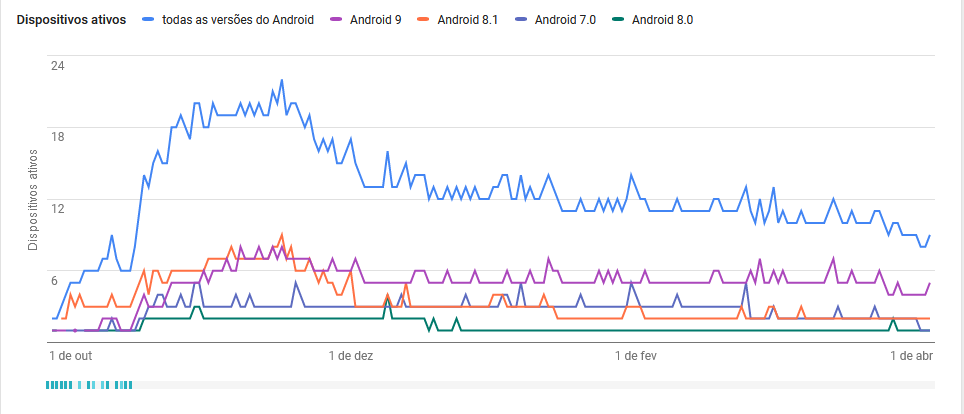
\includegraphics[scale=0.25]{Imagens/taxa_desocupacao.png}
\fonte{\citeonline{ibge_pesquisa_2019}}
\label{figura_2}
\end{figure}

Os alunos graduandos ainda apresentam lacunas de formação em seu potencial empreendedor e que cabe às universidades criar processos de ensino e aprendizagem que preencham esses espaços \cite{pietrovski_alise_2019}. Com as universidades e institutos de ensino superior sendo reconhecidamente contextualizados como promotores da inovação no Brasil, país que configura o 13.º lugar entre os maiores produtores de publicações de pesquisa (\textit{papers}) e inovação ao nível mundial, \citeonline{clarivate_analytics_web_of_research_2017}. 

Logo, as universidades brasileiras precisam se ajustar a esse novo paradigma educacional, que situa as instituições de ensino superior no campo da promoção do empreendedorismo direcional e sistemático, assim como o comportamento empreendedor. A educação empreendedora disciplinada mostra-se eficaz no tocante ao surgimento das inovações, direcionadas e a promoção da identidade empreendedora para novos negócios \cite{jain_academics_2009}. A universidade vem a ser um local privilegiado do saber, da liberdade acadêmica e da experimentação científica, e tem prerrogativa para tornar o empreendedorismo como um conteúdo de conhecimento, e uma ferramenta capaz de gerar inovações \cite{dolabela_oficina_2008}. 


Atualmente, diversas categorias de métodos e ferramentas de ensino podem ser utilizadas para auxiliar o docente e, consequentemente, motivar os estudantes em sua experiência na melhoria das soft skills demandadas pelo mercado de trabalho. Para atingir os objetivos da educação empreendedora, é preciso promover reflexões nos campos do ensino, formação de professores, uso dos recursos e infraestrutura \cite{marques_experiencia_2019}. O desenvolvimento do interesse ao empreendedorismo envolve diversos conteúdos de aprendizado, e é necessário organizar as metodologias e suas aplicações pedagógicas \cite{rocha_avaliacao_2014}. O mesmo autor elencou os Principais Métodos, Técnicas e Recursos Pedagógicos no Ensino do Empreendedorismo.



%\begin{longtable}{p{3.5cm}p{11.0cm}}

%\caption[\textbf{Principais  métodos, técnicas e recursos pedagógicos no ensino de empreendedorismo}]{\textbf{Principais  métodos e recursos pedagógicos no ensino de empreendedorismo}} 
%\label{tabela_2} \\


%\hline \hline \multicolumn{1}{p{3.5cm}}{\textbf{Métodos, Técnicas e Recursos}} & \multicolumn{1}{c}{\textbf{Aplicações}}\\ \hline 

%\endfirsthead


%\multicolumn{2}{c}%

%{{ \bfseries \tablename \ \thetable{} - \ \textbf{Continuação}}}\\
%
%\hline \multicolumn{1}{p{3.5cm}}{\textbf{Métodos, Técnicas e Recursos}} & \multicolumn{1}{c}{\textbf{Aplicações}}  \\ \hline 

%\endhead

%\hline \multicolumn{2}{r}{{\textbf{Continua}}} \\ \hline

%\endfoot
%\hline \multicolumn{2}{r}{{\textbf{Continua}}} \\ \hline

%\endfoot
%\hline \multicolumn{2}{r}{{\textbf{Conclusão}}} \\ \hline
%\hline \hline

%\endlastfoot

%Aulas expositivas & Transferir conhecimentos sobre o Empreendedorismo, as características pessoais do empreendedor, os processos de inovação, fontes de recursos, financiamentos e aspectos legais de pequenas empresas.  \\

%Visitas e contatos com empresas & Estimular o \textit{network} e incitar o estudante a sair dos limites da IES para entender o funcionamento de mercado na vida real.\\

%Plano de negócios & Desenvolver as habilidades de planejamento, estratégia, marketing, contabilidade, recursos humanos, comercialização. Desenvolver a habilidade de avaliação do novo negócio, analisando o impacto da inovação no novo produto ou serviço. Construir habilidade de avaliar e dimensionar riscos do negócio pretendido. \\ 

%Estudos de situações problemas & Construção da habilidade de pensamento crítico e de avaliação de cenários e negócios. Desenvolver a habilidade de interpretação e definição de contextos associados ao Empreendedorismo. \\ 

%Trabalhos teóricos em grupo & Construção da habilidade de aprender coletivamente. Desenvolver a habilidade de pesquisar, dialogar, integrar e construir conhecimentos,buscar soluções e emitir juízos de valor na realização do documento escrito. \\ 

%Trabalhos práticos em grupo & Construção da habilidade de atuar em equipe. Desenvolver a habilidade de planejar, dividir e executar tarefas em grupo, de passar e receber críticas construtivas. Ampliar a integração entre o saber e o fazer.  \\ 

%Grupos de discussão & Desenvolver a habilidade de testar novas ideias. Desenvolver a capacidade de avaliar mudanças e prospectá-las como fonte de oportunidades. \\ 
 
%\textit{Brainstorming}  & Construção da habilidade de concepção de ideias, prospecção de oportunidades, reconhecendo-as como oportunidades empreendedoras. \\ 


%Seminários e palestras com empreendedores & Transferir conhecimentos das experiências vividas por empreendedores desde a percepção e criação do produto, abertura do negócio, sucessos e fracassos ocorridos na trajetória empreendedora. \\ 

%Criação de empresa & Transpor as informações do plano de negócios e estruturar os contextos necessários para a formalização. Compreender várias etapas da evolução da empresa. Desenvolver a habilidade de organização e planejamento operacional. \\ 

%Aplicação de provas dissertativas & Testar os conhecimentos teóricos dos estudantes e sua habilidade de comunicação escrita. \\ 

%Atendimento individualizado & Desenvolver a habilidade de comunicação, interpretação, iniciativa e resolubilidade. Aproximar o estudante do cotidiano real vivido nos pequenos negócios. \\ 

%Trabalhos teóricos individuais & Construção da habilidade de concepção de conhecimento individualizado, estimulando a autoaprendizagem. Induzir o processo de autoaprendizagem. \\ 

%Trabalhos práticos individuais & Construção da habilidade da aplicação dos conhecimentos teóricos individuais, estimulando a autoaprendizagem. Estimular a capacidade laboral e de auto realização. \\ 

%Criação de produto & Desenvolver habilidade de criatividade, persistência, inovação e senso de avaliação. \\ 

%Filmes e vídeos & Desenvolver a habilidade do pensamento crítico e analítico, associando o contexto assistido com o conhecimento teórico. Estimular a discussão em grupo e o debate de ideias. \\ 

%Jogos de empresas e simulações & Desenvolver a habilidade de criar estratégias de negócios, solucionar problemas, trabalhar e tomar decisões sob pressão. Aprender pelos próprios erros. Desenvolver tolerância ao risco, pensamento analítico, comunicação intra e intergrupais. \\ 

%Sugestão de leituras & Prover ao estudante teoria e conceitos sobre o Empreendedorismo. Aumentar a conscientização do ato empreendedor. \\ Incubadoras & Proporcionar ao estudante espaço de motivação e criação da nova empresa, desenvolvendo múltiplas competências, tais como habilidades de liderança, organizacionais, tomada de decisão e compreender as etapas do ciclo de vida das empresas. Estimular o fortalecimento da network com financiadores, fornecedores e clientes. \\

%Competição de planos de negócios & Desenvolver habilidades de comunicação, persuasão e estratégia. Desenvolver capacidade de observação, percepção e aplicação de melhorias no padrão de qualidade dos planos apresentados. Estimular a abertura de empresas mediante os planos vencedores. \\ 

%\end{longtable}
%\fonte{\cite{rocha_avaliacao_2014}}


Os centros de ensino devem contribuir para o desenvolvimento da “cultura empreendedora” por meio da “educação empreendedora ativa” \cite{tscha_empreendendo_2014}, que incentive tanto docentes quanto aos discentes a “despertarem dentro de si o espírito empreendedor e a explorar o espaço potencial para o empreendedorismo, transformando realidades por meio dos empreendimentos que podem desenvolver economicamente e socialmente um país e uma sociedade” \cite{tscha_empreendendo_2014}. Uma vez que, a cultura empreendedora depende diversos fatores influenciáveis ao longo do aprendizado e vida. \cite{dornelas_empreendedorismo_2005} explica que empreender segue fluxo um definido que depende de fatores determinantes durante a construção correta e satisfatória da cultura empreendedora. Alguns fatores estão descritos na figura \ref{figura_2}.

\begin{figure}[H]
\centering
\caption{\textbf{Fatores que influenciam o aprendizado do comportamento empreendedor}}
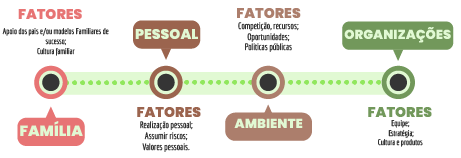
\includegraphics[scale=1]{Imagens/esquema_influencias_empreendedorismo.png}
\fonte{Adaptado de \cite{dornelas_como_2003}}
\label{figura_2}
\end{figure}


Segundo \citeonline{bacich_metodologias_2018} a aprendizagem mais profunda e efetiva, requer espaços de prática frequentes (aprender fazendo) e de ambientes ricos em oportunidades.  São importantes os estímulos interdisciplinares e multissensoriais, tais como o empreendedorismo acadêmico, utilizando para isto as metodologias ativas. Os mesmos autores definem as metodologias ativas como:

\begin{citacao}
Estratégias de ensino centradas na participação efetiva dos estudantes na construção do processo de aprendizagem, de forma flexível, interligada e híbrida. As metodologias ativas, num mundo conectado e digital, expressam-se por meio de modelos híbridos, com muitas possíveis combinações. A junção de metodologias ativas com modelos flexíveis e híbridos traz contribuições importantes para o desenho de soluções atuais para os aprendizes de hoje \cite{bacich_metodologias_2018}.
\end{citacao}

O ensino ativo do empreendedorismo acadêmico, apresenta-se também como uma potencial ferramenta para difusão e transferência de inovação e pesquisa realizadas por acadêmicos oriundos de laboratórios ou, departamentos onde a tecnologia se originou, \cite{guo_what_2019, abreu_nature_2013}. Numa busca de oportunidades e iniciativas utilizando os meios existentes no ambiente acadêmico. Os conteúdos necessários ao efetivo ensino do empreendedorismo vão além da oferta de apenas uma disciplina, sendo preciso que a instituição de educação, a partir de novas práticas pedagógicas, transforme-se em também em uma organização empreendedora \cite{campelli_empreendedorismo_2011}. É necessário dar visibilidade ao ensinamento e promoção do comportamento empreendedor ao aluno com vistas a resolutividade de problemas \cite{degen_o_1989} e despertar da criatividade.

Diante da necessidade de solidificar o ensino empreendedor, que a \textit{Commission Enterprise and Industry Directorate-General} \cite{european_commission_best_2008} estruturou a educação empreendedora direcionada ao ensino superior em três objetivos, representados no modelo esquemático que pode ser visto na Figura \ref{figura_3}, em que se explica às três bases que estruturam os objetivos do ensino do Empreendedorismo no meio acadêmico. 

\begin{figure}[H]
\centering
\caption{\textbf{Pilares do ensino ao empreendedorismo.}}
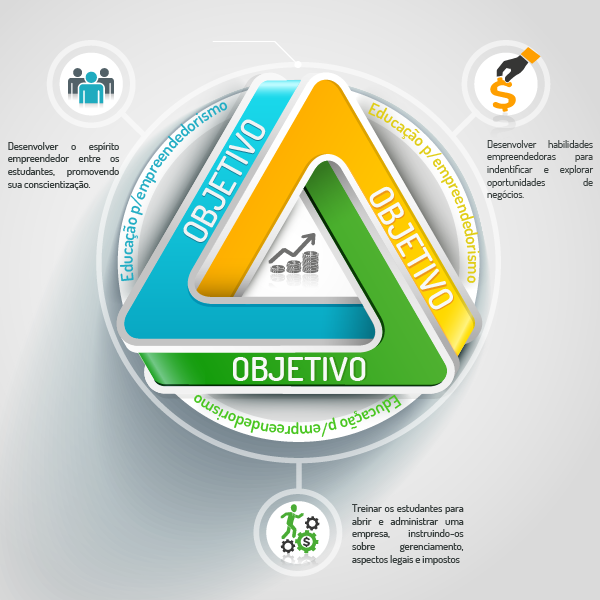
\includegraphics[scale=2]{Imagens/objetivos_educacao_empreendedora.png}
\fonte{Adaptado de \cite{european_commission_best_2008}}
\label{figura_3}
\end{figure}

Como visto, ensino do empreendedorismo perpassa por diversas vertentes, porém, visando a associação de tais conteúdos aos técnicos científicos de forma interdisciplinar, é explorado neste trabalho a proposta de educação empreendedora que tem como base a Aprendizagem Baseada em Problemas (ABP), a Aprendizagem Baseada em Projetos (ABP) \cite{bender_aprendizagem_2015}, que são os passos para elaboração dos conteúdos para o desenvolvimento de um empreendimento bem-sucedido segundo \cite{aulet_empreendedorismo_2019} no livro: empreendedorismo Disciplinado. 

Segundo \citeonline{bender_aprendizagem_2015} a ABP tem como objetivo o desenvolvimento do autoconhecimento com ênfase na perseverança, na imaginação, na criatividade, na inovação, para resolubilidade de problemas reais. É muito importante o conteúdo que se aprende a fazer, mas, sobretudo, o que aprendido \cite{souza_disseminacao_2001}, de forma que a união de tais conhecimentos se some a um melhor desenvolvimento aos profissionais graduados que irão ao mercado de trabalho ou ao mundo dos negócios. O conhecimento científico promovido de forma interdisciplinar na graduação, além de repassar os conhecimentos técnicos, promove uma considerável contribuição para se desenvolver o raciocínio independente, criativo e inovador. Nesse sentido buscamos nesta pesquisa uma abordagem que possa explorar todos os conteúdos de uma metodologia disciplinada e estruturada.

\section{Empreendedorismo Rural Sustentável}

Este trabalho está relacionado com estudo do Desenvolvimento Rural de forma sustentável e circular. Anteriormente, o conceito de Desenvolvimento Rural Sustentável era denominado por “Progresso Rural”, pois, havia um entendido genérico como sentido parcial e prático de “Melhoramento do ambiente” \cite{almeida_da_1995}. Entretanto, torna-se imprescindível destacar que, o desenvolvimento sustentável no meio rural não pode ter suas bases de compreensão apenas no progresso econômico, local ou regional.

É importante compreender que, para melhor incorporar o conceito de sustentabilidade é necessário ter um olhar sistêmico que permeie todo o processo, envolvendo diversas dimensões, dentre as quais se destacam a econômica, a sociocultural, a político-institucional e a ambiental \cite{vieira_politica_2015}. A ação de desenvolvimento sustentável, fruto do avanço social, contribui com a prosperidade da sociedade, ao introduzir inovações anti-predatórias que satisfazem as demandas específicas e pontuais enquanto lidam com a autossuficiência de forma consciente e duradoura. Desta forma satisfazem as necessidades no presente, sem comprometer a capacidade das gerações futuras de suprir suas demandas \cite{onu_sustainable_2016}. 


O meio rural deve ser visto segundo \cite{kageyama_desenvolvimento_2008} como, uma amálgama de práticas heterogêneas, estilos mutuamente contrastantes, tendências de desenvolvimento divergentes, posições hegemônicas e mudanças quase subterrâneas que, a princípio, são praticamente imperceptíveis, mas que, por fim, podem mudar todo o sistema de produção. Compreender a complexidade do rural se faz necessário uma vez que a simples padronização do ambiente é um conceito reducionista do campo, uma maneira concisa do que ocorre no rural \cite{van_der_ploeg_trajetorias_2011}.

O empreendedorismo é uma das ferramentas possíveis para promoção de desenvolvimento do campo e que considera suas complexidades, \citeonline{autio_retaining_2016} afirmam que um euro de financiamento público para as iniciativas em empreendedorismo gerou 1,11 euros de crescimento das vendas excedentes. Para que seja aplicado corretamente, se faz necessário compreender melhor o empreendedorismo sustentável como também a aplicação prática no meio rural. 

Segundo \citeonline{dornelas_como_2003}, o empreendedorismo significa fazer algo novo, diferente, mudar a situação atual e buscar, de forma incessante, novas possibilidades de negociações, tendo como foco a inovação e a criação de valor. Outrossim, \citeonline{leite_aprendizagem_2015} trata o empreendedorismo como um processo, que dedicar-se em iniciar e gerir empreendimentos, isto é, o conjunto de conceitos, métodos, instrumentos e práticas relacionadas com a criação, implantação e gerenciamento de novas empresas ou organizações.

Existem diversas definições de empreendedorismo, mas a essência resume-se na inovação, ou seja, criação de algo novo ou modificação de algo buscando uma nova aplicação. Empreender é empregar os recursos disponíveis de forma criativa, assumindo riscos calculados e buscando oportunidades, ou seja, é um processo de criação de um negócio de valor com recursos limitados tornando-o capitalizável e economicamente viável \cite{costa_empreendedorismo_2006, lopes_educacao_2010}. Apesar dessa diversidade conceitual, a ideia de empreendedorismo tem sido predominantemente associada às concepções de progresso e tecnologia usual deixando de lado o campo e nele suas aplicações práticas.
 
O intenso debate sobre desenvolvimento da agricultura brasileira de forma sustentável em consonância com assuntos econômicos de interesse nacional, torna o tema desta pesquisa oportuno e atual, haja vista que o que se produz na agricultura no Brasil correspondeu a 19\% do total das exportações no ano de 2018 \cite{mdic_comex_2019}. Entretanto, este meio de produção convive com a limitação dos recursos naturais \cite{jacobi_meio_1999}, levando ao Estado pensar em políticas públicas que busquem soluções para as demandas tecnológicas surgidas no meio rural, e gerar profissionais capazes de compreender a complexidade da intensa produção no campo, mantendo o ritmo constante das mudanças tecnológicas ao mesmo tempo em que convivemos com o uso de limitados recursos naturais  \cite{costa_dinamica_2016}.

No alcance desse modelo sustentável, um profissional empreendedor deve ser preparado desde a academia através da educação empreendedora de modo que, ele seja capaz de melhorar o próprio desempenho produtivo \cite{da_silva_qualidade_2017} e a capacidade competitiva\cite{hoffmann_brasil_2015}. Ele deve ser inovador frente as novas demandas \cite{morais_empreendedorismo_2018}. Ao mesmo tempo, garantir a sustentabilidade por meio da manutenção constante de sua principal ferramenta de trabalho, o meio ambiente.

Uma das alternativas possíveis para reduzir os riscos e se manter ativo e produtivo na atividade profissional, é o investimento em tecnologia e inovação tais como: técnicas de desenvolvimento de sementes melhoradas, modelos matemáticos de adubação agrícola mais eficiente, em centros coletivos de pesquisas direcionadas ao campo (para pesquisadores universitários e empresariais), assim como o incentivo ao desenvolvimento de pequenas empresas prestadoras de serviços desenvolvidas por profissionais do meio rural (startups) \cite{bochi_dorneles_coletivos_2014, gomes_inovacao_2014}.
Estes negócios objetivam a melhoria de determinada área agropecuária \cite{volpato_agtechs_2019} ou necessidade do negócio, de forma efetiva e economicamente viável. 

\section{Agritechs}

Quando o ambiente é dinâmico e incerto  com mudanças constantes nos padrões de competitividade e necessidades tecnológicas, a exemplo ao ambiente dos negócios agrícolas, as empresas devem manter também um ritmo de adaptação de seus recursos e rotinas para se manter competitiva independente do tamanho e demanda que venha a ter uma atividade comercial agrícola \cite{koch_reciprocal_2017}. O produtor rural objetivando o desenvolvimento de capital utiliza-se de um vasto aparato de recursos humanos e tecnológicos. A velocidade do desenvolvimento agrícola e conexões das negociações antes realizadas de pessoa a pessoa, atualmente passa pelo campo extremamente automatizado e digitalizado aumentando a velocidade da inovação interferindo na relação entre pessoas e produtividade \cite{campos_o_2016}.

No entanto, os pequenos produtores muitas vezes dependem apenas deles mesmos, sendo proprietário e administrador, ou quando exige a possibilidade de contratação passa a depender de apenas um profissional, responsável por lidar com todos os entraves da produção agrícola e das mudanças constantes do meio rural \cite{soares_relacao_2017}, desta necessidade que atualmente surgem as Startups que no meio rural se apropriaram dos termos “agtechs” e “agritechs”. As startups surgiram por meio das oportunidades que os negócios e as necessidades lhes apresentaram, transformando as inevitabilidades de problemas em ideias e posteriormente em negócios viáveis e sustentáveis. 

As agtechs se ajustaram muito bem ao meio rural já que, para obter sucesso e alcançar o crescimento rápido na produtividade agrícola é necessária uma capacidade de gerar tecnologias adaptativas e ecológicas \cite{contini_hayami_2019}. O modo como se processa a diversificação tecnológica no campo relaciona-se diretamente com o desenvolvimento e a adaptação de novas tecnologias agrícolas e a diversidade das condições socioeconômicas e ambientais \cite{fen-azmeyer_o_2019}. Neste ambiente de cocriação surgem as Startups direcionadas à agricultura. Tais empresas de base tecnológica são focadas em soluções para o agronegócio e muitas vezes são referenciadas como um setor \textit{agtech} \cite{blanco_agtechs_2020}.

Um dos artifícios em ascensão para a melhoria da produção agrícola é a agricultura de precisão, desenvolvida com viés de tecnologia da informação que utiliza dados bases tais como a variabilidade de solo e clima, níveis nutricionais e necessidades de manejo, alcançando desta forma um aumento substancial da produção. Este sistema de interpretação e gestão atenua os custos da produção, aumenta a produtividade do propriedade e diminui erros da colheita com base em dados anteriormente coletados.

A atualmente o Brasil conta com mais de 200 Startups direcionadas aos negócios rurais, que, espectro dos novos empreendimentos, os mais comuns para o agronegócio no Brasil são: \textit{Business to Business} (B2B), \textit{Business to Consumer} (B2C), \textit{Business to Business to Consumer} (B2B2) e o \textit{Direct to Consumer} (D2C). As principais áreas de atuação destas Startups são as áreas de: IoT e Hardware, Software de gestão agrícola, agricultura de precisão e consultoria, a também em crescente expansão a área de alimentos atendendo tanto B2B quanto B2B2C \cite{abstartups_startupbase_2019}, quanto aos fatores de desenvolvimento de uma Agritechs no Brasil segundo \cite{mondin_2_2018} está na observação de iniciativas de outros negócios e vivências práticas, demonstrando que a vivência do ambiente rural e experimentações de programas que incentivem ao surgimento de novos negócios é de suma importância para o surgimento de mais empreendimentos.


\section{Propriedade Intelectual no Meio Rural}

A criatividade presente na mente humana gerou inúmeras, reformulações da natureza a partir de resoluções de problemas que surgem a partir da evolução das interações sociais, ela surge no meio de uma inquietação relacionada com algum problema existente no território em que a inovação está inserida. \cite{pacheco_dos_2018}. Desta forma, atualmente toda criação advinda do intelecto humano, tais como música, produto, processo, nova cultivar, desenhos, artigos científicos, trabalhos literários ou artísticos constituem um ativo, bem ou direito \cite{costa_interseccao_2011}. Tais ativos sendo eles registrados ou não, estão ligados diretamente ao seu autor/inventor sendo isto considerado direito de propriedade intelectual. Este direito vai muito além da inovação \cite{wipo_tratado_1970}, mas a relação entre o seu autor/inventor e sua respectiva criação intelectual.

Para proteção aos possíveis direitos econômicos oriundos das produções intelectuais torna-se desejável que essas inovações e tecnologias sejam depositadas e patenteadas quando tais inovações satisfazem as requisições de registro industrial. Marcadamente quando pertencente aos campos de invenção, ou publicação de ideias e premissas e quando tais inovações pertencerem aos campos de registro de Direito Autoral \cite{wipo_b06_2019}. 

Aliadas às ações para o desenvolvimento de inovações, o inventor ou autor deve ter certa atenção as Propriedades Intelectuais que tangem seu produto, ou processo. Sendo assim, é visível que há uma grande afinidade entre estes dois temas, principalmente os direitos que cabe ao meio industrial e dos autores ligados a “softwares”. A crescente interação comercial, financeira e tecnológica entre a economia e seus agentes exigem padrões modernos de proteção para a PI, uma vez que os direitos sobre os nomes empresariais, tecnologias, \textit{designs}, marcas, entre outros, representam valiosos ativos das empresas e profissionais autores/inventores \cite{sherwood_propriedade_1992}. 

Nesse contexto, o sistema de propriedade intelectual permite incentivar a geração de novas tecnologias, produtos e processos, tal como, promover a criação de empresas inovadoras em todas as áreas de informação, uma vez que concede ao autor/inventor explorar economicamente suas produções. Da mesma forma que os países com melhor proteção de Direito de Propriedade Intelectual (DPI), atraem significativamente mais atividades, fusões e aquisições transnacionais de alta tecnologia. Isto ocorre particularmente nas tidas como emergentes economicamente, proporcionando um ganho maior de aporte estrangeiro para desenvolvimento tecnológico interno \cite{hasan_impacts_2017}, e registro de novas patentes.

A patente e as publicações científicas, representam instrumentos jurídicos de proteção do invento resultante de um esforço de pesquisa das instituições de pesquisa, e de pesquisadores no desenvolvimento de processos tecnológicos e novos produtos. Isto torna um investimento seguro, rentável e legítimo se prevenindo do comportamento desleal que podem surgir da concorrência, evitando a comercialização resultante de cópia não permitida, aspecto que desrespeita o esforço realizado pelos detentores originas e os gastos implicados no desenvolvimento \cite{marques_natureza_2017}.

O conceito de Propriedade Intelectual é amplo e difere de país a país, em suma pode ser entendido como, à área do Direito que, garante a inventores ou responsáveis por qualquer produção do intelecto, seja nos domínios industrias, científicos, literários ou artísticos, o direito de obter, por um determinado período, recompensa pela própria criação \cite{aspi_aspi_2019}.

O princípio de independência dos direitos inseridos no ordenamento jurídico internacional, possibilita que matéria protegida seja considerada de domínio privado podendo converter-se em um produto ou processo com garantias outorgadas no país registrado, e pelo qual os demais interessados terão de pagar direitos de uso \cite{galvao_direitos_2002}. Se mostra importante a busca da compreensão atual das propriedades intelectuais e inovações tecnológicas à luz das áreas derivadas dos contextos dos recursos hídricos, de modo a compreender o contexto e caminho do desenvolvimento tecnológico.

O amparo legal e necessário para garantir que os investimentos em pesquisa e desenvolvimento retornem ao inventor, provocando um processo cíclico positivo, em que maiores investimentos em PD seriam promovidos diante da concessão do monopólio temporário de exploração do invento \cite{lima_sauglobal_2017}. No Brasil a PI é composta por três grandes áreas: propriedade Industrial, Direito do Autor e Suis generis, demais ramificações podem ser vistas na Figura \ref{figura_4}.


\begin{figure}[H]
\centering
\caption{\textbf{Modalidades da propriedade intelectual no Brasil}}
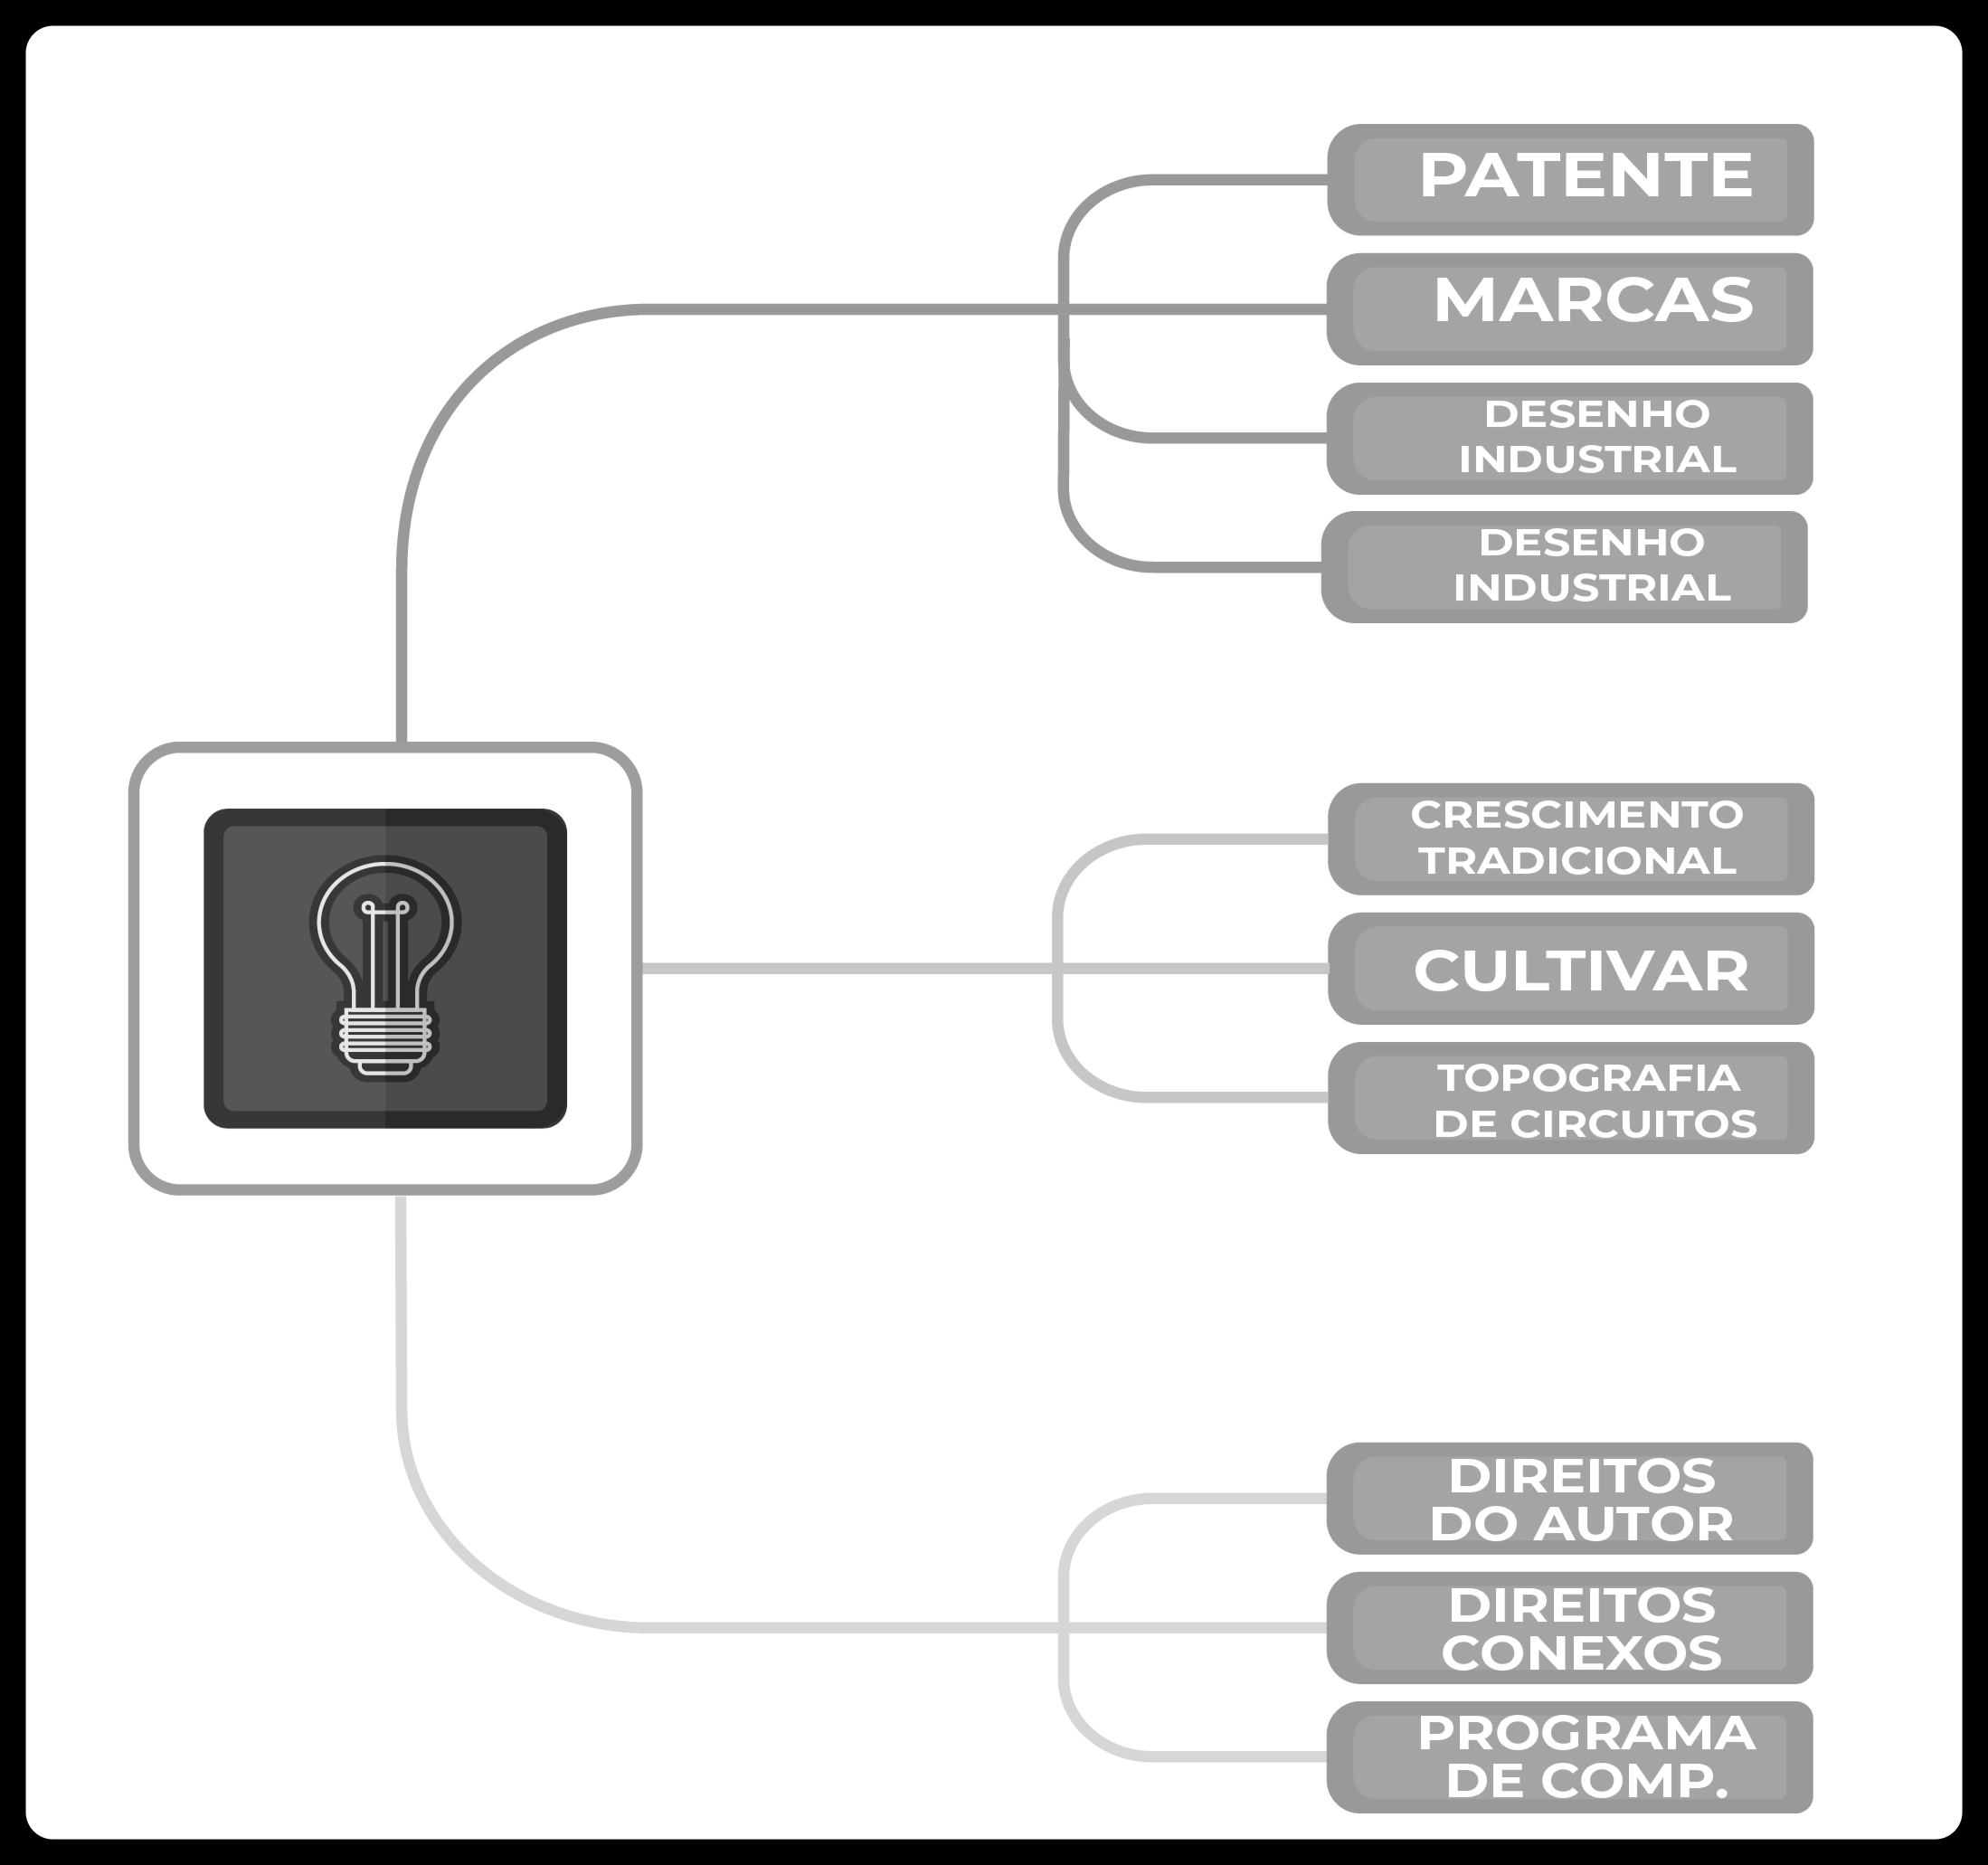
\includegraphics[scale=0.8]{Imagens/propriedade_intelectual.png}
\fonte{Adaptado de \cite{inpi_manual_2017}}
\label{figura_4}
\end{figure}


Os documentos que compõem os pedidos de patente são constituídos por diferentes partes: relatório descritivo, reivindicações e resumo \cite{inpi_diretrizes_2011}. Por sua natureza redacional, deve descrever todo o objetivo, funcionalidades e reivindicações das proteções solicitadas, se mostrando um texto capaz de demonstrar quais os aspectos da invenção e quais os pontos inéditos que trazem esta novidade industrial, expressando desta forma possíveis inovações \cite{wipo_global_2018}.  


Diante de tais mudanças sobre o cenário do desenvolvimento tecnológico e das Propriedades Intelectuais (PI) surgem inúmeras questões sobre o papel que os sistemas de registro e divulgação para PI desempenham no desenvolvimento da sociedade que está vinculada e o incentivo à inovação deste \cite{segala_os_2016}. Os países que apresentam uma economia mais forte, dispõe de um sistema de proteção de propriedade mais robusto e confiável, concomitantemente, uma maior quantidade de registros e depósitos das mais variadas finalidades \cite{mueller_universidades_2014}.


